\section{Bilder Begrüßungsabend WS2022/2023}
\sectionmark{Bilder Begrüßungsabend WS2022/2023}

%\begin{figurehere}
%	\begin{center}
%		\includegraphics[width=\linewidth]{Bilder/andechs2.jpg}
%%		\caption{xxx} 
%	\end{center}
%\end{figurehere}


\begin{multicols}{2}
Als eine der auffälligsten Veranstaltungen im Wintersemester in unsere geliebte Vandalia finden wir das Martinsgansessen, das eine perfekte Gelegenheit bietet, mit der Familie daran teilzunehmen und dieses Wintersemester 2023/2024 ist keine Ausnahme. Dank unsere AH Michael Oppitz und Richard Gurtner und die Organisation der Chargen konnten wir eine Abend mit leckerem Essen, Bundesbruder und Familien aus erster Hand genießen. Der Tag begann frühmorgens mit der Essenszubereitung. Dank der Erfahrung unserer älteren Herren und der Hilfe einiger Bundesbrüder war es kein großes Problem, alles für die Gänse zum Backen für den Rest des Nachmittags bereitzuhalten und so den charakteristischen Geschmack zu erhalten, den wir später probieren würden. Als alles fertig war, mussten wir offensichtlich nur noch ein paar Bier öffnen, um auf die gute Arbeit anzustoßen. Mit der Ankunft von mehr AH und Familien war die Atmosphäre immer besser geworden. Die Zeit für das Abendessen rückte immer näher so war es nur noch die Aufgabe der Aktive Bundesbruder die kneipesaal für alle unsere Gäste fertig einzurichten und zu dekorieren. Es war schon 19 Uhr und konnte man immer mehr bekannte Gesichter sehen, die mit einem Lächeln und einem Bier zur Begrüßung aller Gäste eintrafen. Gleichzeitig konnte man einige Kinder sehen, die im Vorraum und kneipesaal herumliefen und ihre Mütter, die sie gewarnt haben, darauf aufzupassen, sich nicht zu verletzen. Das hat Vandalia in dieser Nacht mit Leben erfüllt und uns allen eine schone Familiäre Atmosphäre verliehen. Als man durch die Küche gehen konnten bereits den Duft der fertigen Gänse riechen, der unserem Appetit anregte. Jetzt mussten wir nur noch das Fass Bier anschließen, das unseren Durst für den Rest des Nachmittags stillen würde, und die Füchse servieren lassen die Gläser Bier und das Essen an diesem Abend. Etwas verspätet begann das Abendessen, ohne dass der Senior zuvor ein paar Dankesworte an alle Gäste für ihre Anwesenheit an diesem Abend und an alle, die an der Zubereitung des Essens beteiligt waren, richtete. Der Abend begann mit einem Gebet vor dem Essen. Man konnte in den Augen aller Anwesenden die Begeisterung sehen, jetzt ihr Essen zu probieren. Für diejenigen, die das Martinsgansessen zum ersten Mal erlebt haben, darunter auch für mich, war es eine angenehme Überraschung, den köstlichen Geschmack der von unserem AH zubereiteten Gans probieren zu können, und für diejenigen, die bereits bei früheren Gelegenheiten dabei waren, war es eine Freude wieder in diesem Semester da zu sein. Zwischen Bier und Gelächter war die gute Stimmung, die damals herrschte, spürbar. Auf der AH-Seite der Tische konnte man sehen, wie sie zusammen mit ihren Frauen und Kindern miteinander redeten, und auf der anderer konnte man die Aktiven sehen, wie sie miteinander Witze machten und wie sich die Biergläser leerten. Der Abend neigte sich dem Ende zu und ich kann für alle sprechen, wenn ich sage, dass wir alle zufrieden waren und wieder eine schöne Erinnerung hatten. Während AH langsam in ihre Häuser zurückkehrten, setzten die Aktiven wie üblich die Nacht fort, bis ein paar Stunden später. Am Ende der Nacht, während sich alle zum Ausruhen zurückzogen, blieb eine schöne Erinnerung an diese Nacht zurück und mit dem Wunsch, nächstes Jahr auf jeden Fall wiederzukommen, um noch einmal die köstliche Gans zu probieren, die wir nur in unserer geliebten Vandalia finden. Als Cosenior dieses Semesters kann ich sagen, dass es eine Nacht war, bei deren Organisation ich mit großer Freude mithelfen konnte, da diese Art von Abenden meiner Meinung nach diejenigen sind, die am meisten geschätzt werden, wenn man sich immer daran erinnert.
\end{multicols}
	
	\begin{figurehere}
		
			%\includegraphics[width=.9\linewidth]{Bilder/ki/01}
			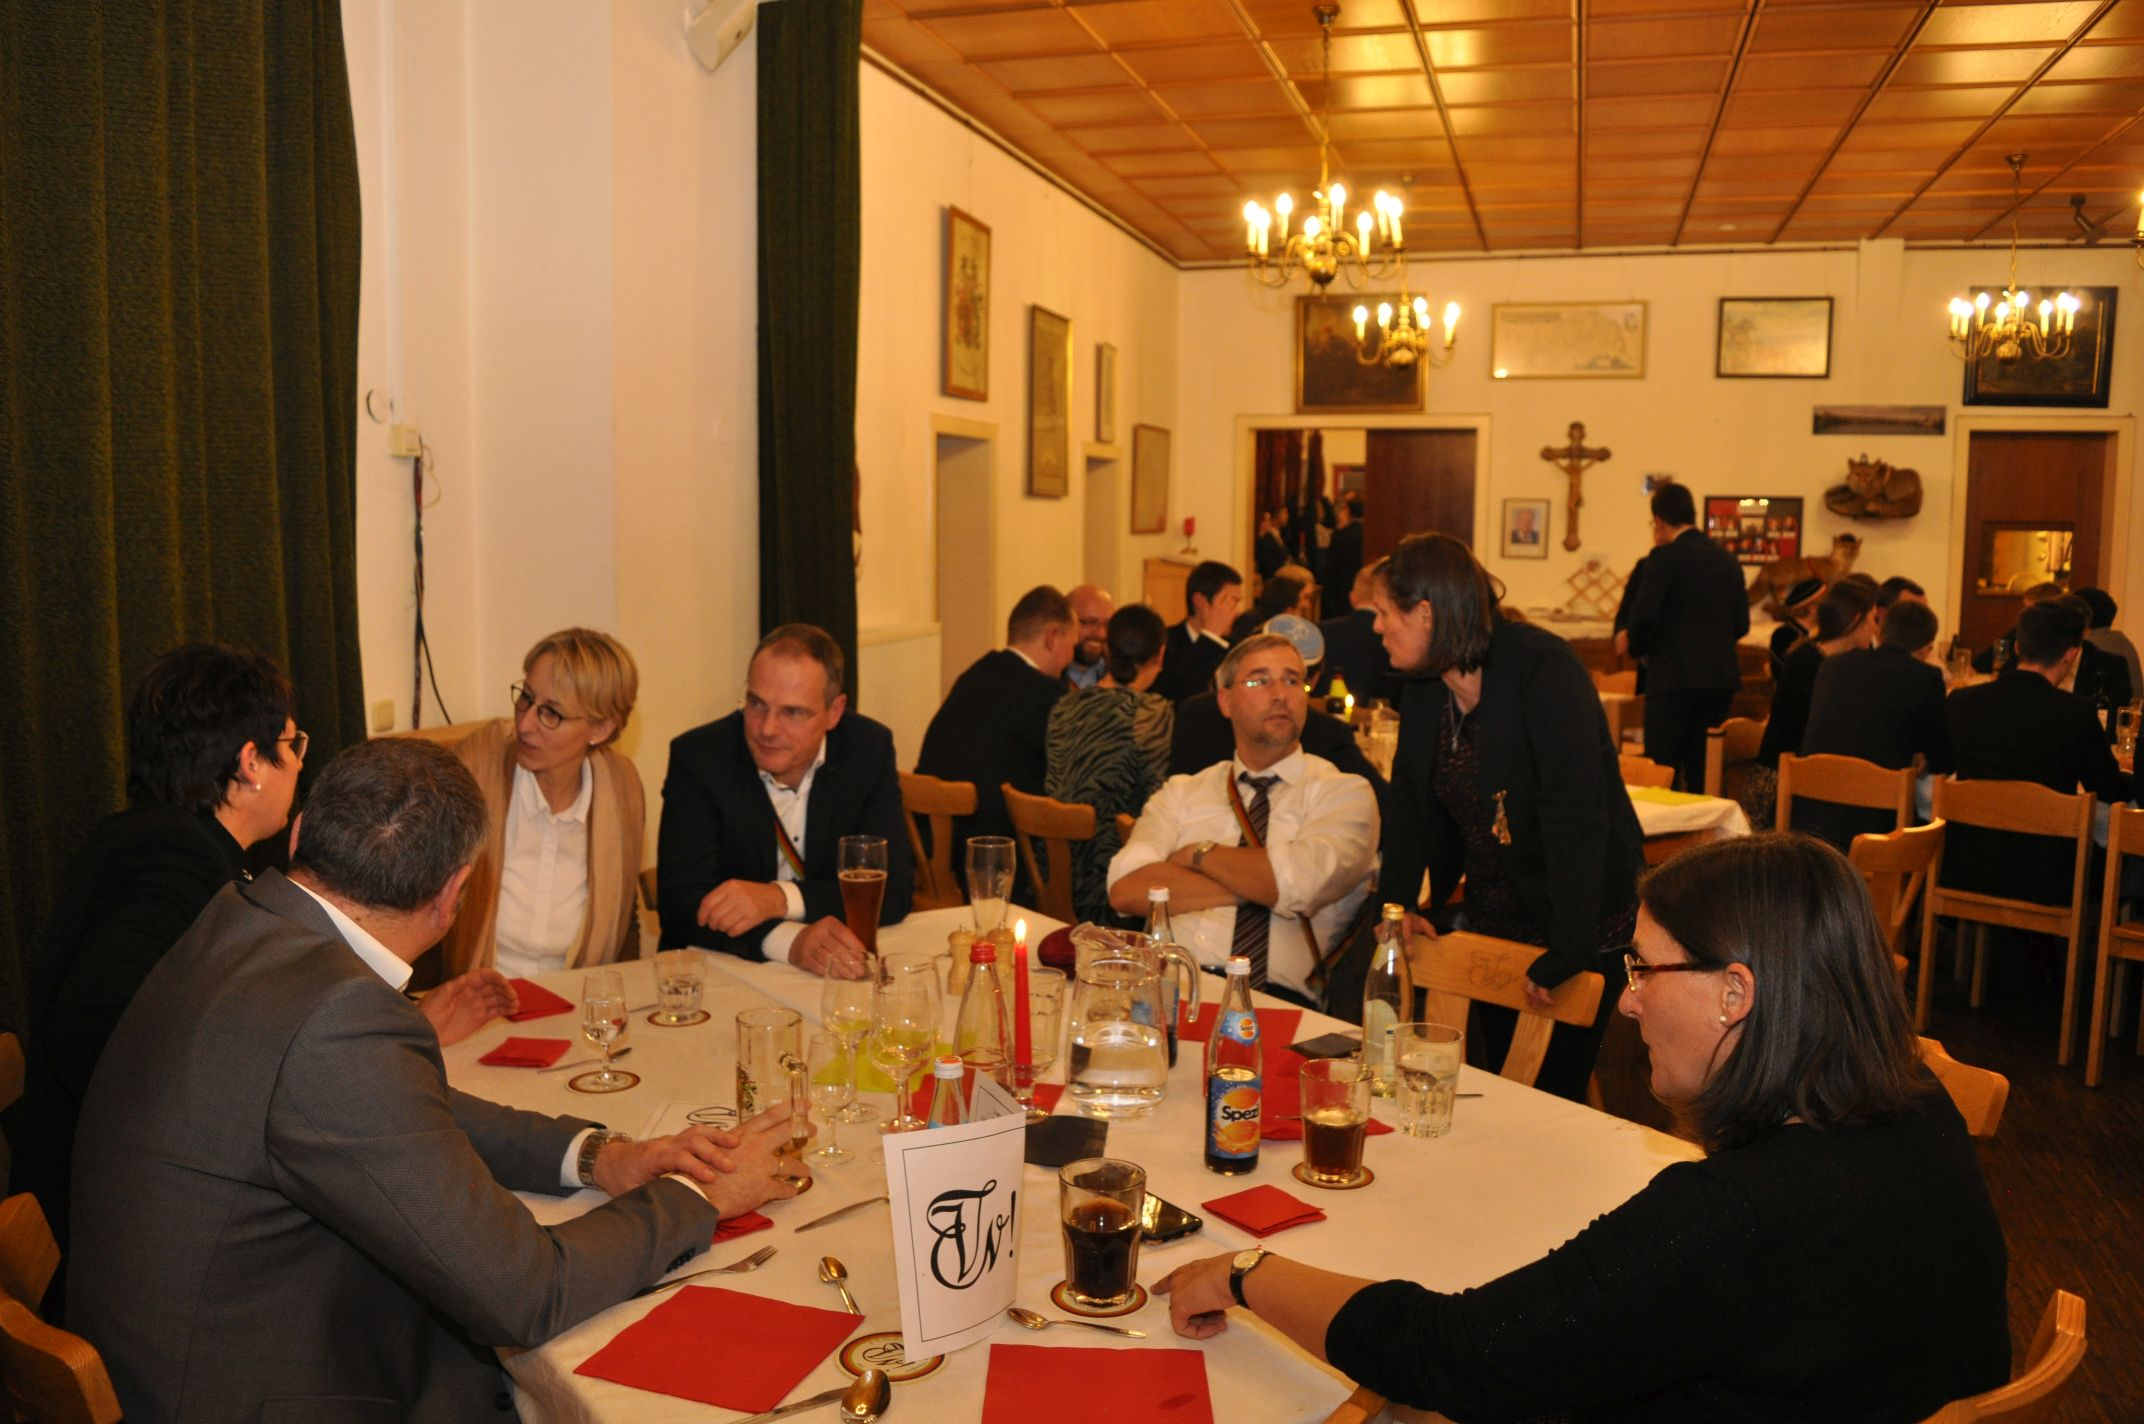
\includegraphics[width=.45\linewidth]{Bilder/begrüßungsabend/Begrüßungsabend-WS2022 (1).JPG}
		   	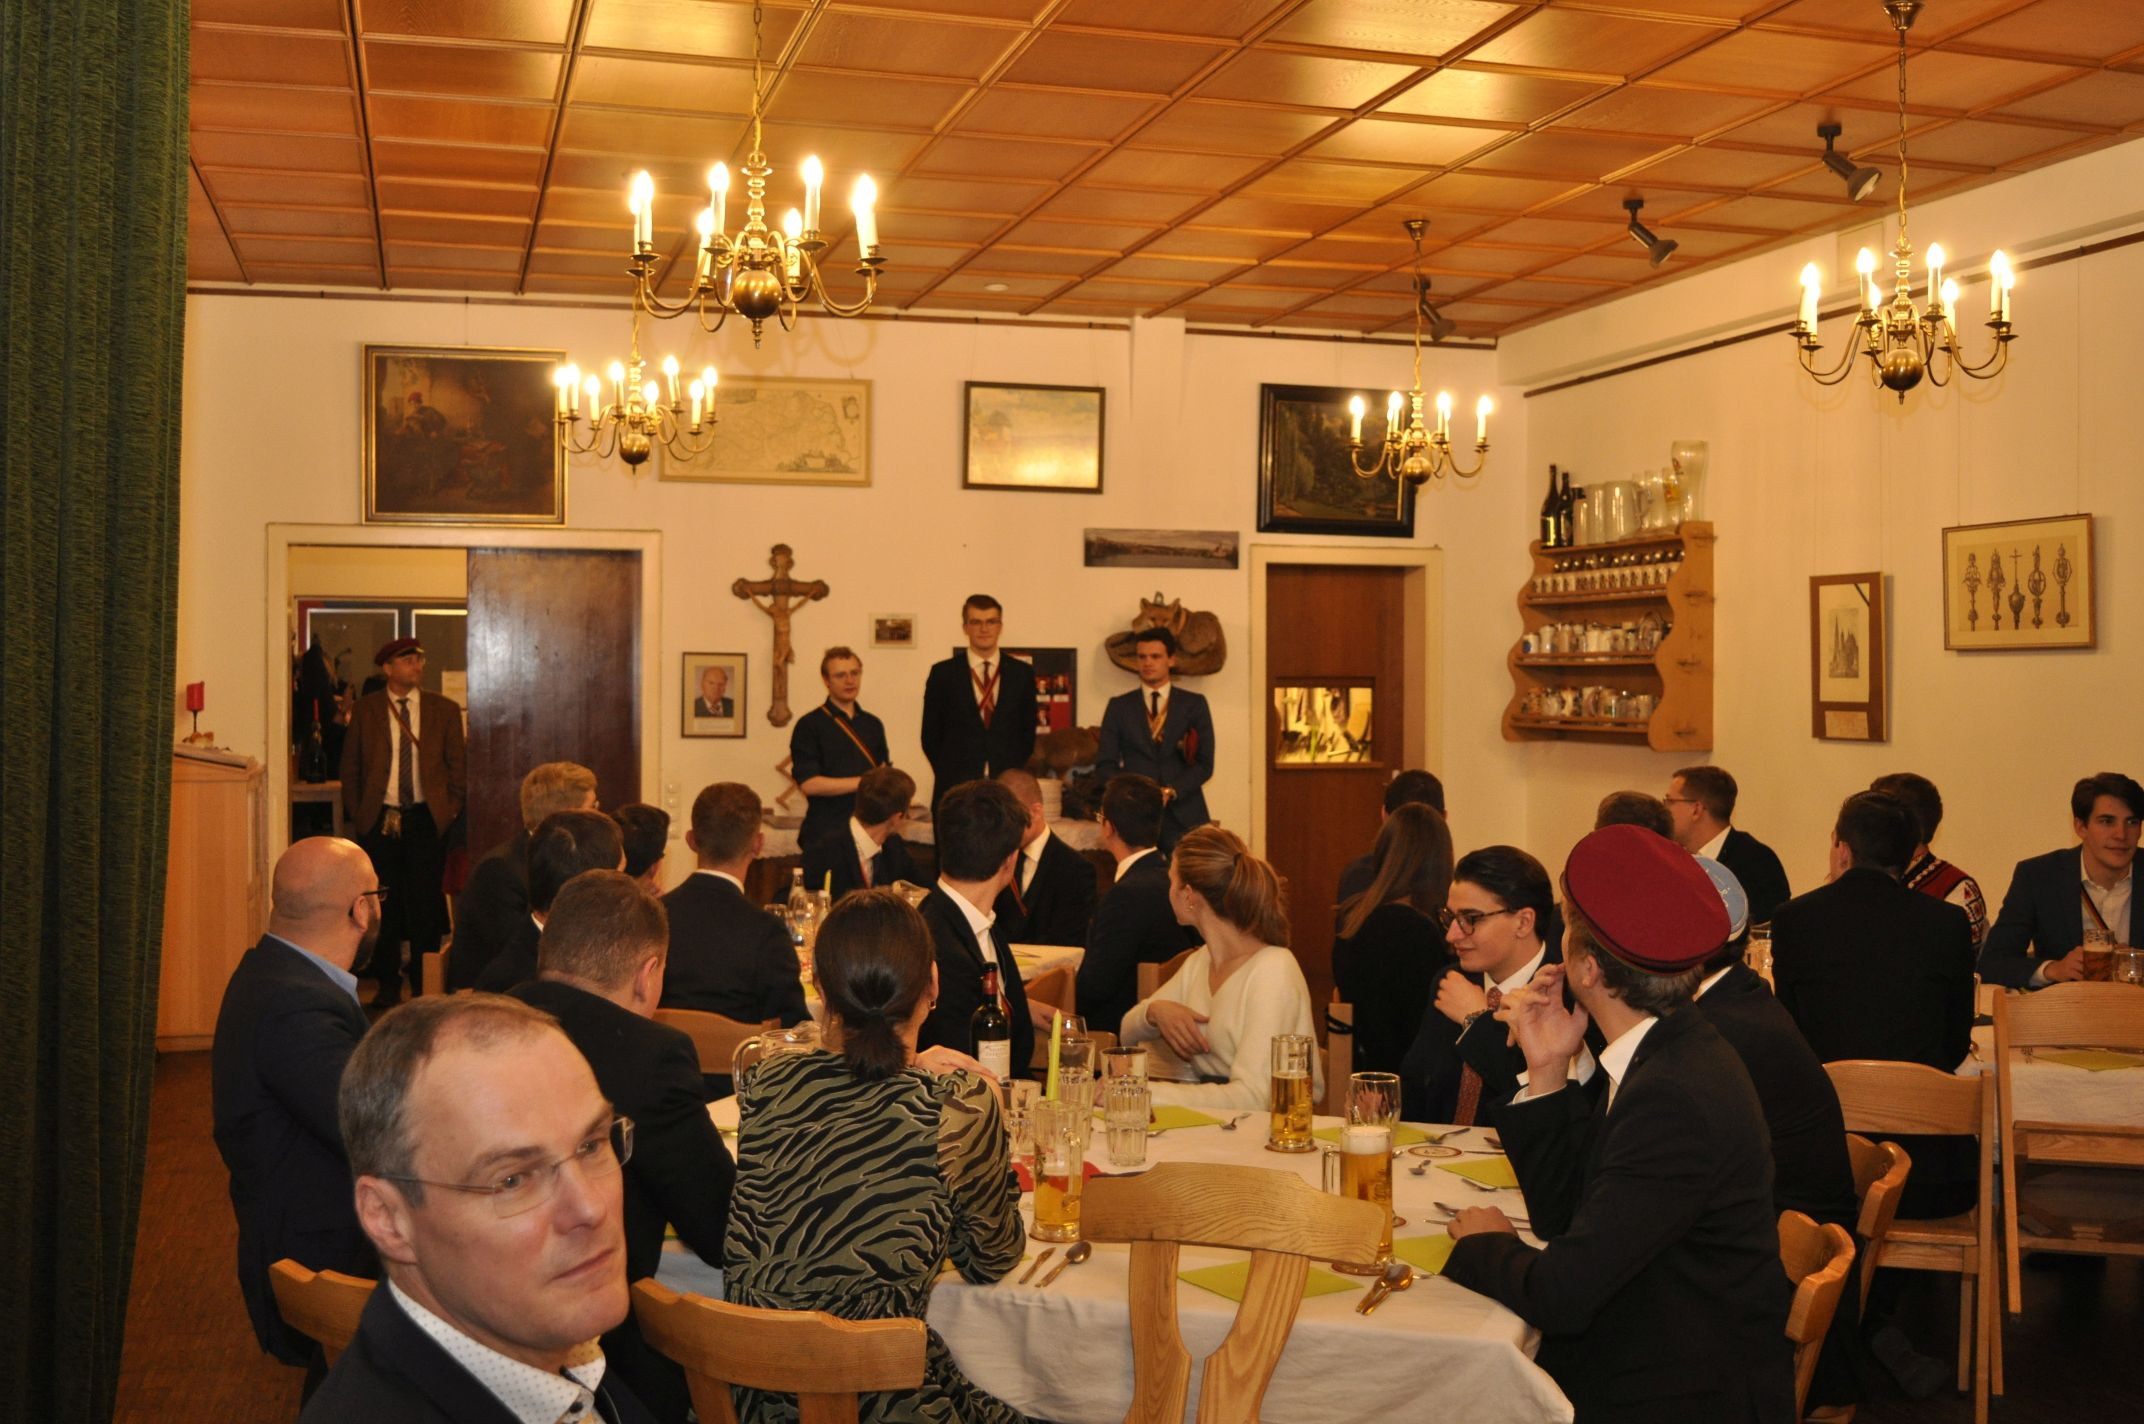
\includegraphics[width=.45\linewidth]{Bilder/begrüßungsabend/Begrüßungsabend-WS2022 (2).JPG}
		   	
		   		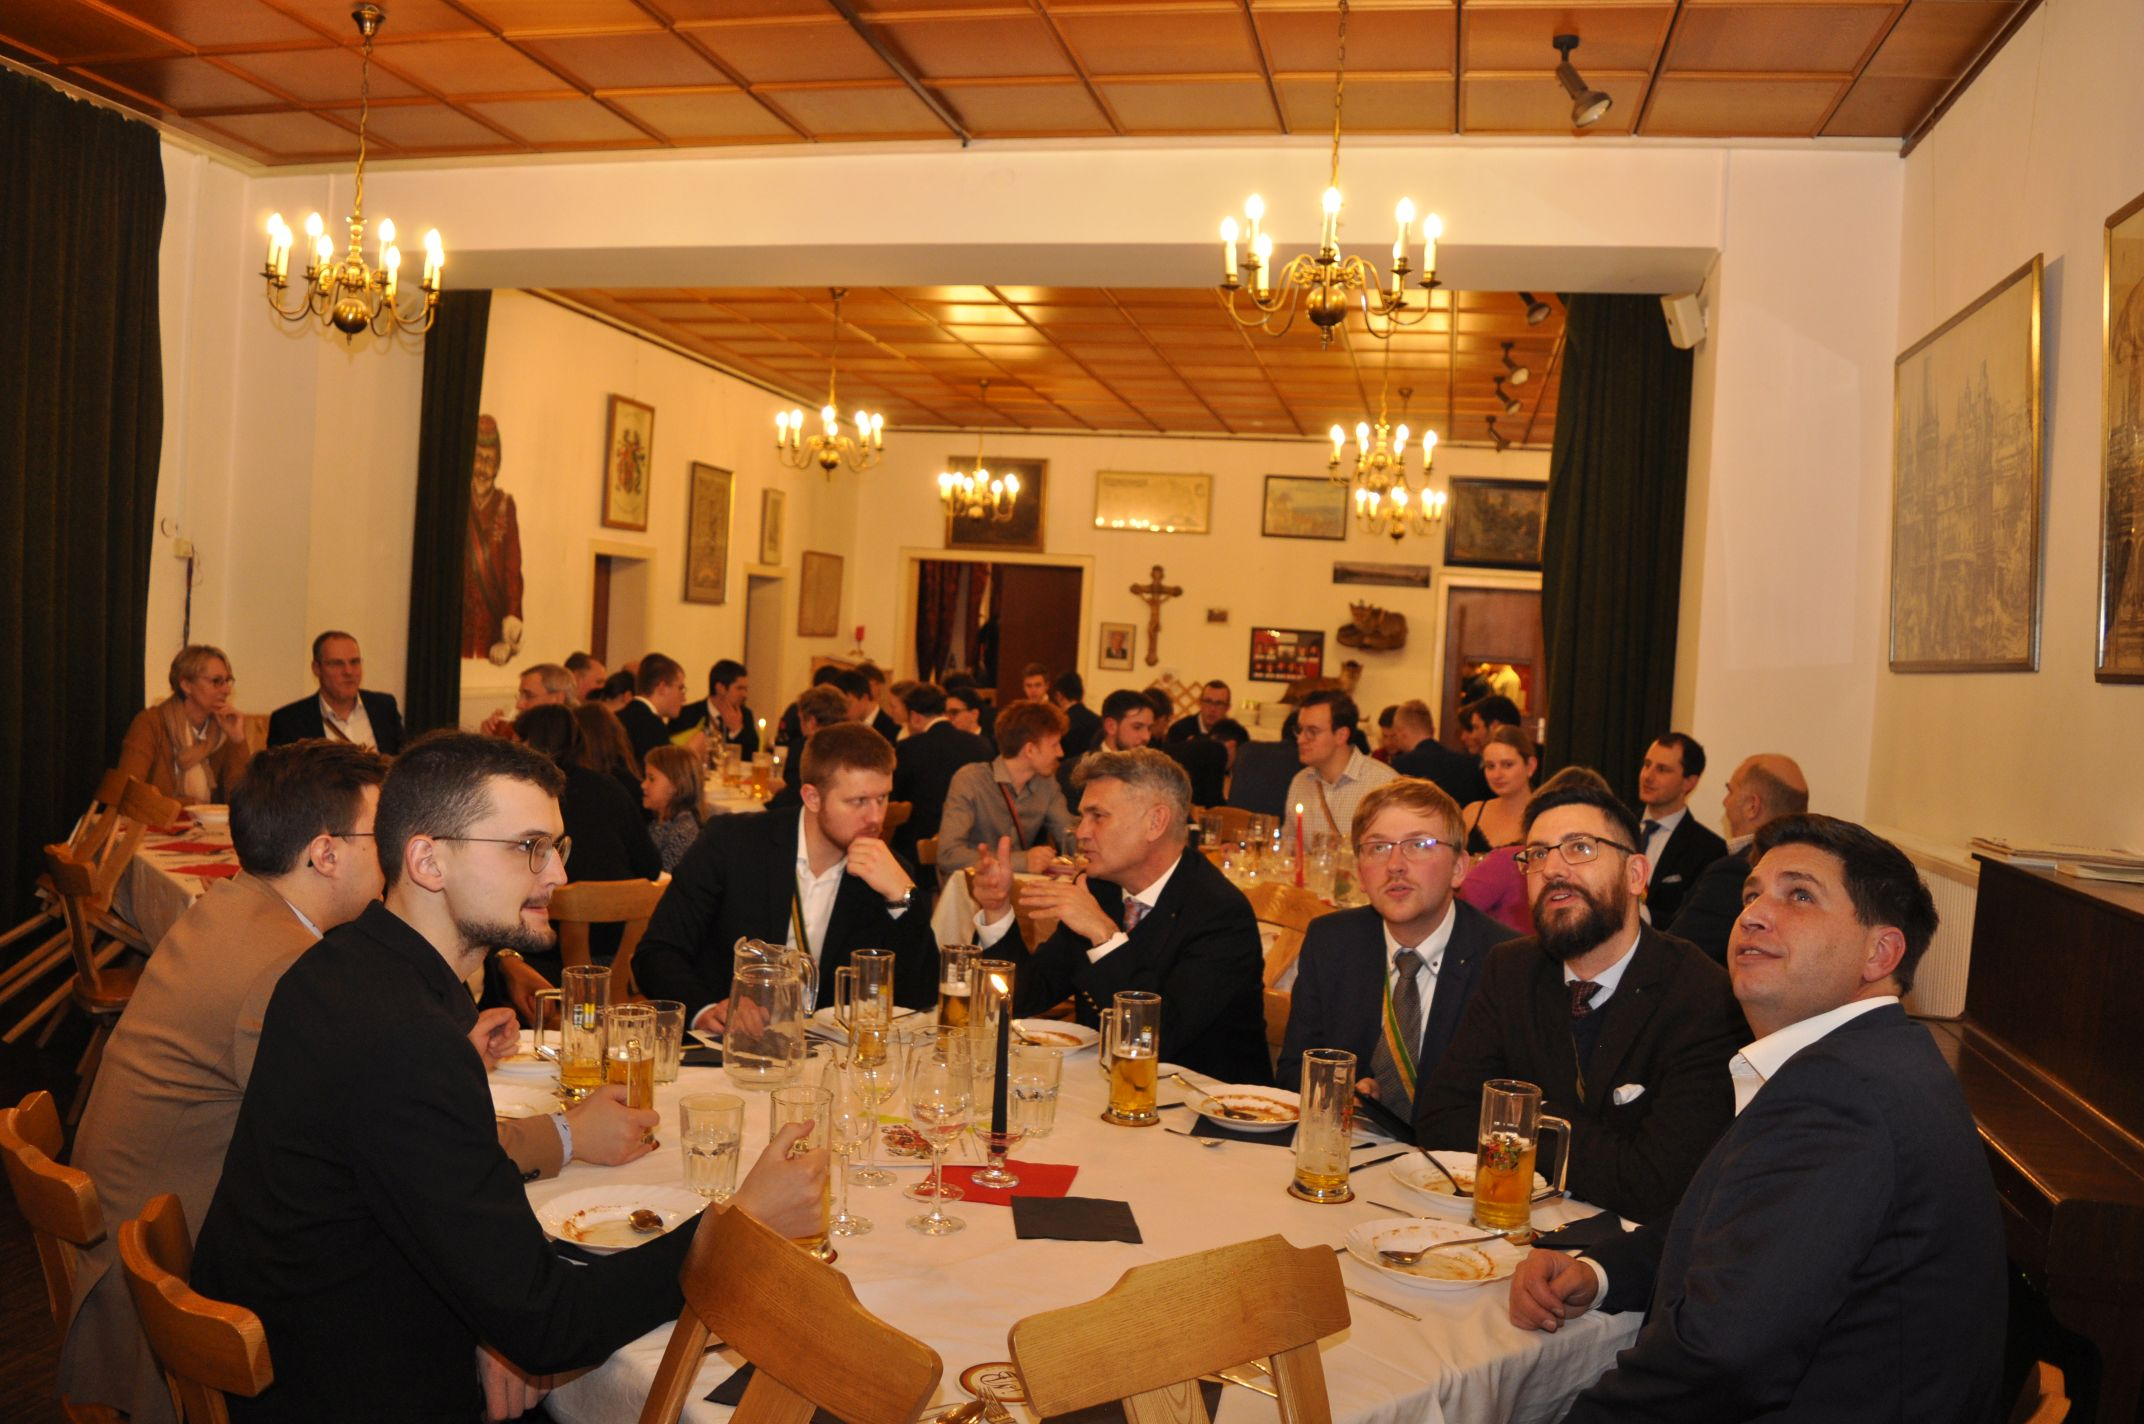
\includegraphics[width=.45\linewidth]{Bilder/begrüßungsabend/Begrüßungsabend-WS2022 (3).JPG}
		   			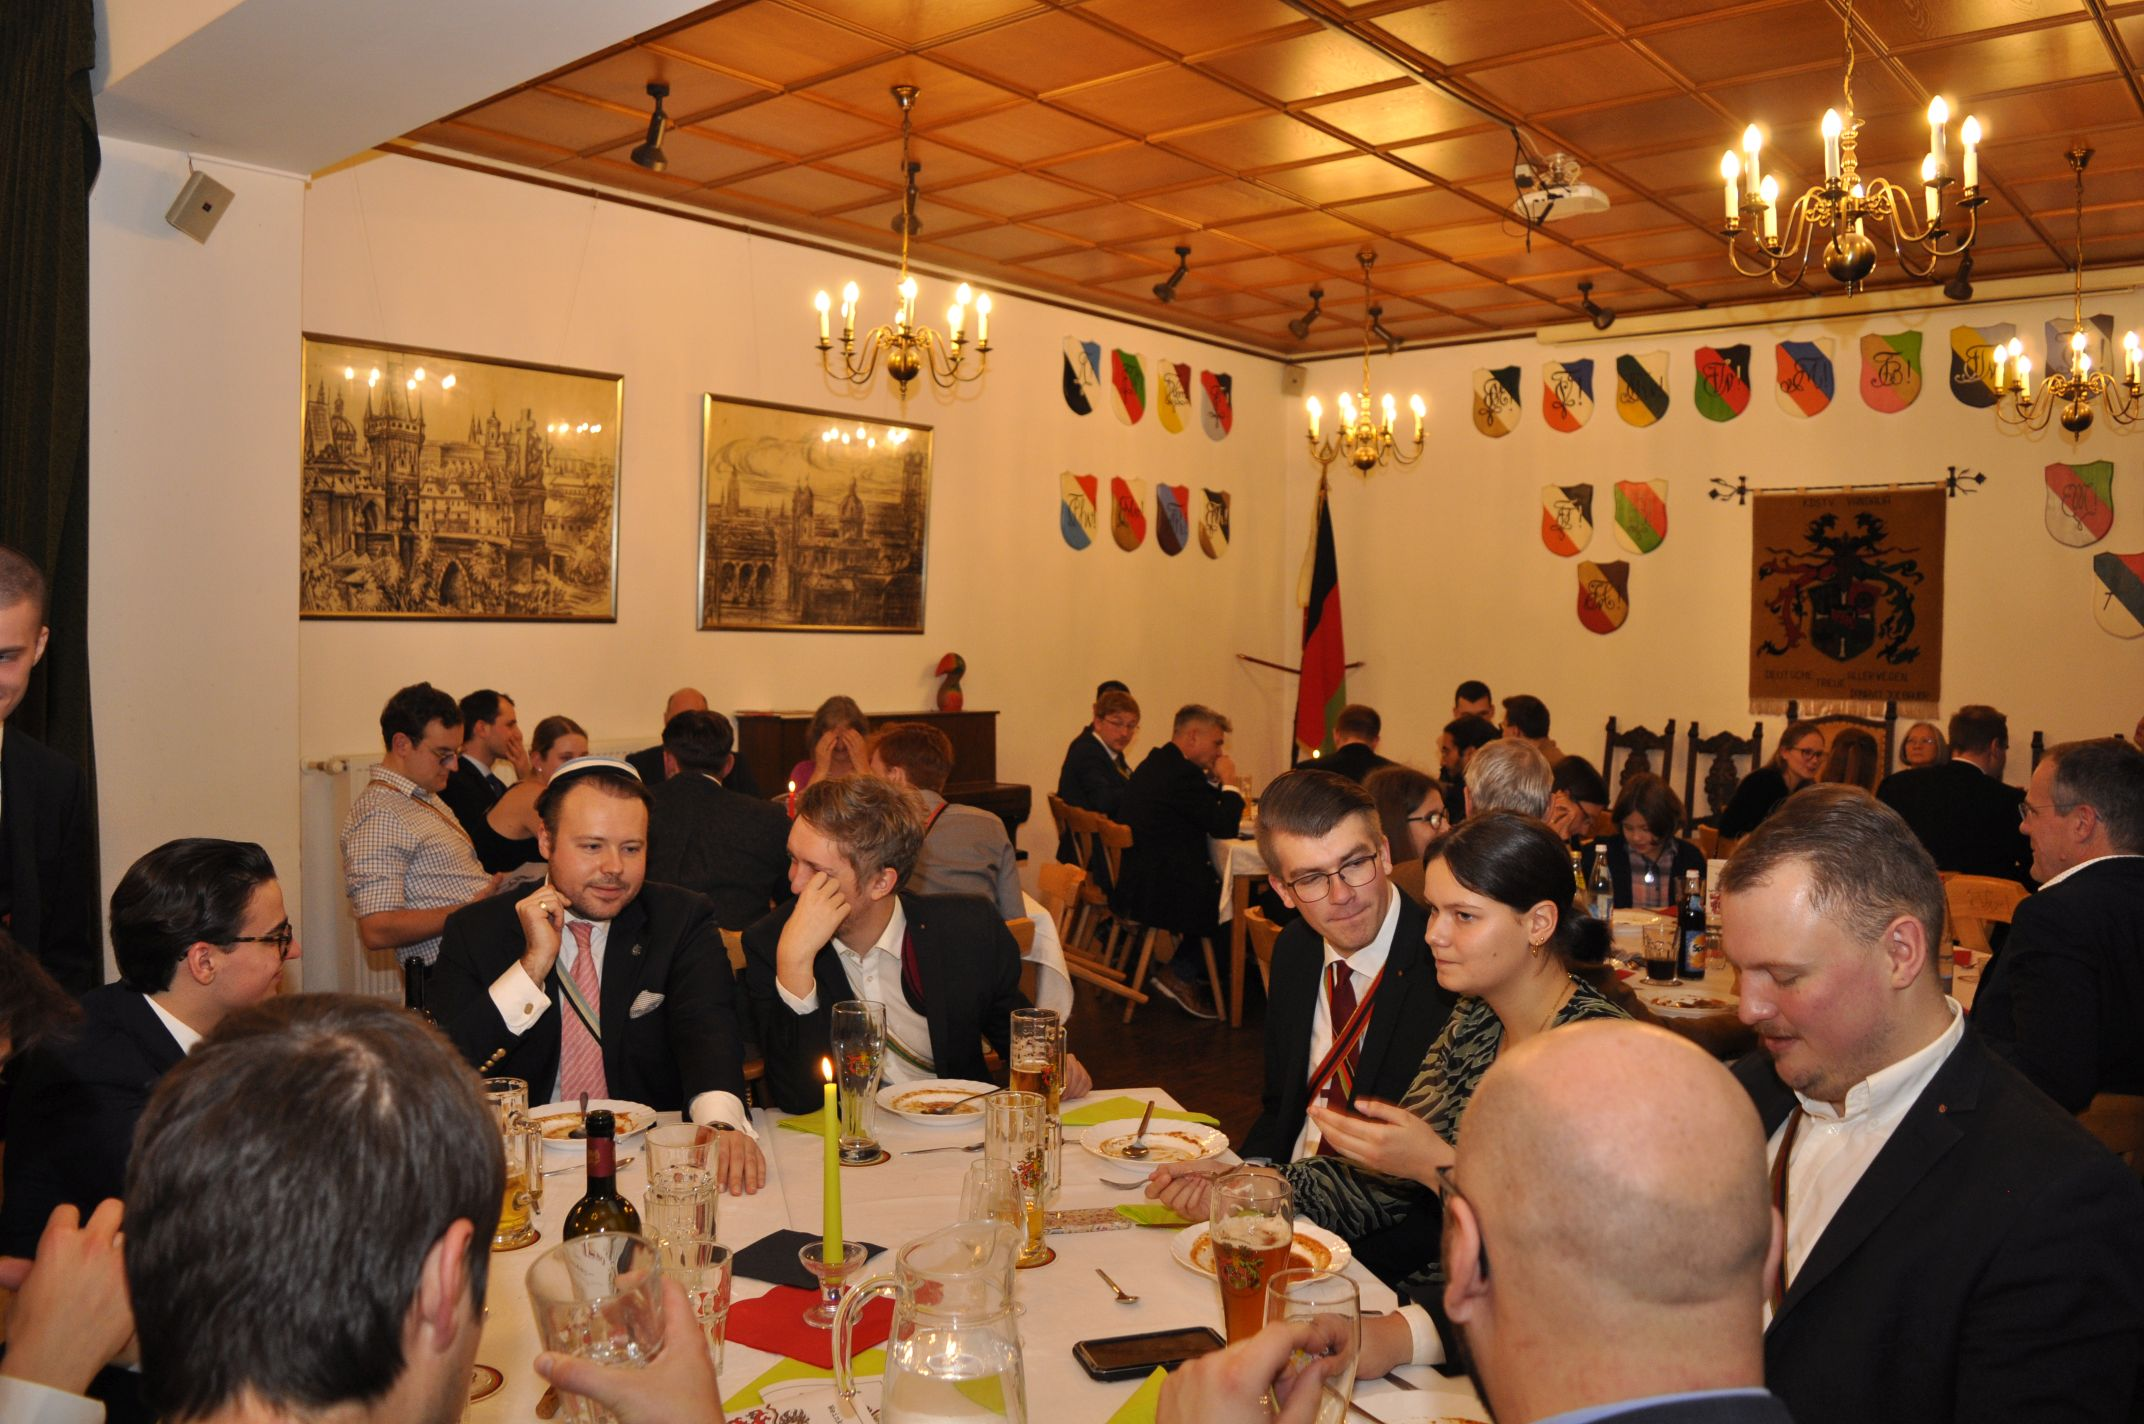
\includegraphics[width=.45\linewidth]{Bilder/begrüßungsabend/Begrüßungsabend-WS2022 (4).JPG}
		   
		   
		    
	\end{figurehere}
	

	

%
%\begin{figurehere}
%	\begin{center}
%		\includegraphics[width=.8\linewidth]{Bilder/pios2}
%		\caption{Realer Aufbau} 
%	\end{center}
%\end{figurehere}